\chapter{Introduction}


\section{Artificial Neural Networks}

	Neural Networks takes a large number of training examples, and then develop a system which can learn from those training examples. By increasing the number of training examples, the networks learn more and improves the accuracy.\\
	
	Along the way, we'll first define artificial neurons and next, learning algorithm for neural network called stochastic gradient descent and a fast way to compute gradient of the cost function (Backpropagation).

\subsection{Artificial Neurons}
\subsubsection{Perceptron Neuron}

	A perceptron takes several binary inputs, $x_1$, $x_2$, $x_3$,.. and gives single binary output. Futher, every input $x_i$ has a weight $w_i$ expressing importance of the respective input. The neuron's output is determined by comparing the weighted sum $\sum_{i} w_{i}x_{i}$ with some threshold value of the neuron. In algebraic terms:
	$$
	output=
	\begin{cases}
	0 if \sum_{i}w_{i}x_{i} \leq threshold \\
	1 otherwise
	\end{cases}
	$$
	
	Further simplifying, we write weighted sum $\Sigma_{i}w_{i}x_{i}$ as a dot product w $\cdot$ x and replace threshold with negative of bias, b. So, the perceptron rule can be rewritten as:
	$$
	output = 
	\begin{cases}
	0 if w \cdot x + b \leq 0\\
	1 if w \cdot x + b \textgreater 0
	\end{cases}
	$$
	The bias can be seen as measure of how easy it is to get perceptron to fire.
				
\subsubsection{Sigmoid Neuron}

	Sigmoid neurons are similar to perceptrons, but modified so that small change in their weights and bias cause only slight revision in their output.
	So, instead of 0 or 1, the inputs can also take on any value between 0 and 1. The output is defined as $\sigma(w \cdot x + b)$, where $\sigma$ is called sigmoid fuction and is defined as:\\*
	$\sigma(x)$ = 1/(1+exp(-z))\\
	Explicitly,
	\begin{equation} 
	output = \frac{1}{1 + exp(- w \cdot x - b)}
	\end{equation}
	
	The sigmoid function is chosen as the smoothness of $\sigma$ means that small change in $\delta w_{j}$ in weights and $\delta b$ in bias will produce small change $\delta output$ from neuron.\\
	From calculus:\\
	\begin{eqnarray} 
	\Delta \mbox{output} \approx \sum_j \frac{\partial \, \mbox{output}}{\partial w_j}
	\Delta w_j + \frac{\partial \, \mbox{output}}{\partial b} \Delta b,
	\end{eqnarray}
	

	The neuron gives a probable idea that a complex network of perceptrons could make quite accurate decisions which may consists of multiple layers of neurons. In this way, many layer network can make a sophisticated decision making.
	

\subsection{Architecture}

	\begin{center}
		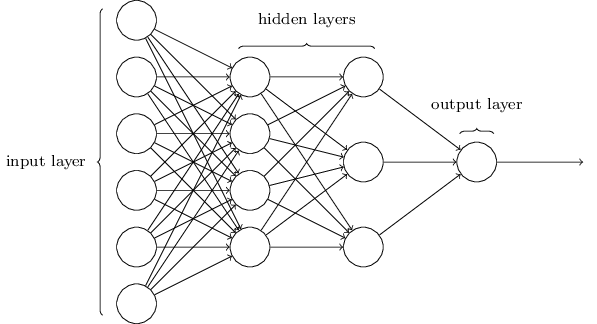
\includegraphics[width=0.75\textwidth]{architecture.png}
	\end{center}

Such multiple later networks are called multilayer perceptrons or MLPs.
As one layer is used as input to the next layer, such networks are called feedforward neural networks.